% How accurately must the IA power spectra be known for Roman cosmic shear?
% Tolerance bands of the GI and II spectra against a 0.3 sigma shift of
% (Omega_m, S8), from the FLAMINGO-stitched truth injected into cosmolike.
% Build with the summary-notes skill: assets/build_note.sh notes/ia_tolerance_bands
\documentclass[11pt]{article}

\usepackage[margin=1in]{geometry}
\usepackage{amsmath}
\usepackage{amssymb}
\usepackage{graphicx}
\usepackage{booktabs}
\usepackage{xcolor}
\usepackage[font=small,labelfont=bf,labelsep=period]{caption}
\usepackage[hidelinks]{hyperref}

% Let figures share pages with text instead of leaving float-only pages.
\renewcommand{\topfraction}{0.85}
\renewcommand{\bottomfraction}{0.7}
\renewcommand{\textfraction}{0.12}
\renewcommand{\floatpagefraction}{0.8}

% Symbols, one macro per object.
\newcommand{\hMpc}{\,h\,{\rm Mpc}^{-1}}
\newcommand{\kuv}{k_{\rm UV}}
\newcommand{\FoB}{{\rm FoB}}
\newcommand{\PNL}{P_{\rm NL}}
\newcommand{\PdE}{P_{\delta E}}
\newcommand{\PEE}{P_{EE}}
\newcommand{\T}{^{\mathsf{T}}}
\newcommand{\bvec}[1]{\boldsymbol{#1}}

% =====================================================================
% Numbers
% =====================================================================
% Part 1: results (analysis/roman_dchi2/v7/tolerance_bands.json, written
% by v7/tolerance_bands.py on 13 November 2026). Part 2: inputs.
%
% Statements of the text that rest on Part 1; re-check after a rerun:
%   - at K_0 = 0.3 the guaranteed band is 1 to 3% at k <= 0.2 for GI and
%     II, and the spectra are unconstrained above about 2 h/Mpc (Summary;
%     "The bands at the production cut");
%   - the guaranteed box is 10 to 16% of the single-node tolerance
%     ("Two bands");
%   - full refits agree with the linear response within 8% for NLA
%     ("Is linear response enough?").
\newif\ifnumbersfinal
\numbersfinaltrue
\newcommand{\refresh}[1]{\ifnumbersfinal#1\else\textcolor{red}{#1}\fi}
% ---------------------------------------------------------------------
% Part 1: results.
% K_0 = 0.3, case A, NLA refitted: single-node and guaranteed bands
% (results[mask = K0/D 0.3, case A, model NLA].bands), percent
\newcommand{\SingleLowLo}{\refresh{8}}     % GI and II separately, k <= 0.2
\newcommand{\SingleLowHi}{\refresh{37}}
\newcommand{\JointLowLo}{\refresh{1}}
\newcommand{\JointLowHi}{\refresh{5}}
\newcommand{\JointBothLo}{\refresh{0.6}}   % GI and II together, k <= 0.2
\newcommand{\JointBothHi}{\refresh{2}}
\newcommand{\JointMidGI}{\refresh{6 to 7}} % GI, k = 0.3 to 0.6
\newcommand{\JointOneGI}{\refresh{23}}     % GI at k = 1
\newcommand{\JointOneII}{\refresh{34}}     % II at k = 1
% guaranteed / single ratio over every configuration (share/0.3)
\newcommand{\RatioLo}{\refresh{0.10}}
\newcommand{\RatioHi}{\refresh{0.16}}
% verification at K_0 = 0.3, case A (bands.<X>.verify)
\newcommand{\VerNLALo}{\refresh{0.306}}
\newcommand{\VerNLAHi}{\refresh{0.325}}
\newcommand{\VerTATTLo}{\refresh{0.24}}
\newcommand{\VerTATTHi}{\refresh{0.36}}
\newcommand{\VerTATTCorner}{\refresh{0.14}}
% baseline FoB of the stitched truth itself, case A, NLA / TATT
\newcommand{\BaseTwo}{\refresh{0.13 / 0.08}}
\newcommand{\BaseThree}{\refresh{0.29 / 0.23}}
\newcommand{\BaseFour}{\refresh{0.31 / 0.27}}
\newcommand{\BaseFive}{\refresh{0.33 / 0.27}}
% the all-points baseline: chi2 and FoB of NLA (first run, log)
\newcommand{\AllChi}{\refresh{2134}}
\newcommand{\AllFoB}{\refresh{22}}
% checks
\newcommand{\PartitionCheck}{\refresh{6\times10^{-10}}}
\newcommand{\BuildCheck}{\refresh{1.1\times10^{-3}}}
% ---------------------------------------------------------------------
% Part 2: inputs.
\newcommand{\Nnodes}{13}
\newcommand{\Threshold}{0.3}

\begin{document}

\begin{center}
  {\LARGE How accurately must the IA spectra be known?\par}
  \vspace{0.6em}
  {\large Tolerance bands of the GI and II power spectra for Roman cosmic
    shear\par}
  \vspace{0.6em}
  {\large November 2026\par}
  \ifnumbersfinal\else
    \vspace{0.6em}
    {\color{red}Numbers in red are being refreshed.\par}
  \fi
\end{center}
\vspace{1em}

\section{Summary}
\label{sec:summary}

\paragraph{The question.}
If the intrinsic-alignment (IA) power spectra entering Roman cosmic shear
are wrong by a fraction $\varepsilon(k)$ that may differ from scale to
scale, how large may $\varepsilon(k)$ be before the best-fit $(\Omega_m,
S_8)$ moves by more than $\Threshold\,\sigma$? The answer is a band in the
$(k, \varepsilon)$ plane, and it is the physical input a scale cut needs:
a model may be used on the scales where its error lies inside the band.

\paragraph{The answer.}
With the production mask $\kuv = 0.3/D(z)$ and the production covariance
(Figures~\ref{fig:nla} and~\ref{fig:tatt}), changing one scale at a time,
Roman tolerates errors of \SingleLowLo{} to \SingleLowHi\% in GI or II at
$k \le 0.2\hMpc$. If every scale may be wrong at once, in the worst
combination of signs, the guaranteed tolerance is \JointLowLo{} to
\JointLowHi\% at $k \le 0.2$, \JointMidGI\% for GI at 0.3 to $0.6\hMpc$ and
\JointOneGI\% at $1\hMpc$; GI and II wrong together must be accurate to
\JointBothLo{} to \JointBothHi\% on large scales. Above about $2\hMpc$
the mask removes the information and any error is allowed. NLA and TATT
give nearly the same bands.

\paragraph{How.}
The truth is FLAMINGO's alignment spectra stitched to NLA on large scales,
injected into cosmolike at the FLAMINGO cosmology. The spectra are
perturbed by tent functions at \Nnodes{} nodes in $k$; because $\xi_\pm$ is
linear in the injected spectra, each node's effect on the data vector is
computed exactly, and the shift of the refitted parameters follows by
linear response. In the plane of whitened $(\Omega_m, S_8)$ every node is
an arrow, and the worst case over all combinations has a closed form
(Section~\ref{sec:bands}). Full non-linear refits at the band edges agree
with the linear response within 8\% for NLA and 20\% for TATT
(Section~\ref{sec:verify}).

\paragraph{Limits.}
The perturbations are the same at every redshift; the truth is one
simulation; and the shift is measured on top of the bias the stitched truth
already produces (figure of bias \BaseThree{} for NLA / TATT at this mask),
so the bands answer ``how much more error is tolerable'', not ``how much in
total''.

\section{Setup}
\label{sec:setup}

\paragraph{The truth.}
The FLAMINGO D3A cosmology ($\Omega_m = 0.306$, $10^9 A_s = 2.099$,
$n_s = 0.967$, $H_0 = 68.1$, $\Omega_b = 0.0486$), CAMB with Takahashi
halofit. The IA spectra are the FLAMINGO measurements stitched to NLA on
large scales: per snapshot, with $R_X = P_X/\PNL$,
\begin{equation}
  R_X(k) = \left[1 - w(k)\right] R_X^{\rm NLA} + w(k)\, R_X^{\rm FL}(k),
  \qquad
  w(k) = \frac{1}{1 + \exp\!\left[-\ln(k/k_t)/0.3\right]},
  \label{eq:stitch}
\end{equation}
for $X = \delta E$ (GI) and $EE$ (II). $R^{\rm NLA} = (-C_1, C_1^2)$ comes
from an NLA fit to FLAMINGO on $0.05 \le k \le 0.3\hMpc$, $R^{\rm FL}$ is a
smoothing spline of the measured ratios, and the transition scale $k_t(z)$
runs from 0.16 to $0.27\hMpc$ over $0.2 \le z \le 2$. Below $k_t$ the truth
is NLA, above it FLAMINGO.

\paragraph{Injection.}
The spectra enter cosmolike as tables (the sim-IA path, IA code 3, built
without trimming the tables), which share the Limber integrals, the
Hankel transforms and the $n(z)$ with the models; the data vector is
\begin{equation}
  \bvec d = \bvec\xi_{GG} + \bvec\xi_{\rm IA}[\PdE, \PEE],
\end{equation}
Roman $\xi_\pm$ in 8 tomographic bins and 15 angular bins, 1080 points.

\paragraph{Analysis.}
The production covariance \texttt{example1\_cov} (Gaussian plus connected
non-Gaussian), the production masks $\kuv(z) = K_0/D(z)$ (an angular bin is
kept when less than 5\% of its signal comes from $k > \kuv$), and cosmolike's
own NLA ($A_1, \eta_1$) or TATT ($A_1, \eta_1, A_2, \eta_2, b_{\rm TA}$)
refitted with every parameter free: $\Omega_m$ and $A_s$ (case A), plus
$n_s$, $H_0$, $\Omega_b$ with Gaussian priors (case B, in the appendix).

\section{Perturbing the spectra scale by scale}
\label{sec:basis}

Pick nodes $k_1 < \dots < k_N$, log spaced from $0.01$ to $10\hMpc$
(\Nnodes{} nodes, four per decade), and the tent functions $h_j(k)$: each
is 1 at its node, falls linearly in $\ln k$ to 0 at the neighboring nodes,
and the end tents stay at 1 beyond the end nodes. A perturbation of the
spectrum $X$ is
\begin{equation}
  P_X(k, z) \;\to\; P_X(k, z)\left[1 + \sum_{j=1}^{N} \varepsilon_j\, h_j(k)\right],
  \label{eq:pert}
\end{equation}
the same at every redshift, so $\varepsilon(k)$ is the piecewise-linear
curve through the values $\varepsilon_j$. Two properties make this basis
convenient.
\begin{itemize}
  \item The tents sum to one at every $k$, so $\varepsilon_j = \varepsilon$
    for all $j$ is a uniform change of amplitude. Numerically, the node
    responses summed over $j$ reproduce $\bvec\xi_{\rm IA}$ to
    $\PartitionCheck$.
  \item $\bvec\xi_{\rm IA}$ is linear in the injected spectra (a Limber
    integral of $P$, then a Hankel transform), so
    \begin{equation}
      \delta\bvec d = \sum_j \varepsilon_j\, \bvec r_j,
      \qquad \bvec r_j \equiv \bvec\xi_{\rm IA}\!\left[P_X h_j\right],
    \end{equation}
    is exact: one cosmolike evaluation per node gives the response $\bvec
    r_j$ for any size of $\varepsilon_j$.
\end{itemize}
Three spectra are perturbed: GI alone, II alone, and both with the same
$\varepsilon_j$. A wrong galaxy bias $b(k)$ in the conversion $\PdE = P_{hE}/b$
is a GI perturbation of the opposite sign, so the GI band covers it.

\section{From a perturbation to a parameter shift}
\label{sec:response}

Let $\bvec m(\bvec p)$ be the model and $\bvec p_0$ its best fit to the
unperturbed truth, with $\chi^2(\bvec p) = (\bvec d - \bvec m)\T C^{-1}
(\bvec d - \bvec m)$ plus Gaussian priors $\Pi$. Adding $\delta\bvec d$ moves
the minimum by $\delta\bvec p$. Expanding $\bvec m(\bvec p_0 + \delta\bvec
p) \simeq \bvec m(\bvec p_0) + J\,\delta\bvec p$ with the Jacobian $J =
\partial\bvec m/\partial\bvec p$ and setting the gradient of $\chi^2$ to zero
gives the normal equations, whose solution is
\begin{equation}
  \delta\bvec p = F^{-1} J\T C^{-1}\,\delta\bvec d,
  \qquad F = J\T C^{-1} J + \Pi^{-1},
  \label{eq:response}
\end{equation}
the Gauss--Newton estimator. It neglects one term of the exact
second derivative of $\chi^2$, $\sum_a (d - m)_a\, [C^{-1}\partial^2 m]_a$,
which is small when the model fits the data; Section~\ref{sec:verify}
tests it.

Only $\bvec\theta = (\Omega_m, S_8)$ matters for the figure of bias. With
$G = \partial\bvec\theta/\partial\bvec p$ and the marginalized covariance
$\Sigma = G F^{-1} G\T$, the figure of bias of a perturbation is
\begin{equation}
  \FoB = \sqrt{\delta\bvec\theta\T\,\Sigma^{-1}\,\delta\bvec\theta}
  = \Bigl|\, \sum_j \varepsilon_j\, \bvec L_j \Bigr|,
  \qquad
  \bvec L_j = \Sigma^{-1/2}\, G F^{-1} J\T C^{-1}\, \bvec r_j .
  \label{eq:fob}
\end{equation}
This is the picture to keep in mind: in the plane of whitened $(\Omega_m,
S_8)$, where the $1\sigma$ contour is the unit circle, each node is a fixed
arrow $\bvec L_j$, a perturbation adds the arrows with weights
$\varepsilon_j$, and the threshold is the circle of radius 0.3. The
model's IA parameters are refitted inside $F$: a perturbation that looks
like a change of $A_1$ is absorbed and gives a short arrow.

\section{Two bands}
\label{sec:bands}

\paragraph{One node at a time.}
If only node $j$ is wrong, $\FoB = |\varepsilon_j|\,|\bvec L_j|$, and the
tolerance is
\begin{equation}
  |\varepsilon_j| < \frac{0.3}{|\bvec L_j|}.
\end{equation}
This band says how sensitive Roman is to each scale, but it is not safe:
two nodes each at their own edge can add up to more than 0.3.

\paragraph{Every node at once: the guaranteed box.}
Ask instead for bounds $b_j$ such that every combination with
$|\varepsilon_j| \le b_j$ stays below 0.3. The largest figure of bias over
that box has a closed form in two dimensions. The length of a vector is
its largest projection on a unit vector, $|\bvec v| = \max_{\phi}
\bvec u_\phi\cdot\bvec v$ with $\bvec u_\phi = (\cos\phi, \sin\phi)$; the two
maximizations can be swapped, and for a fixed direction the box is
maximized node by node by choosing each sign to align with $\bvec u_\phi$:
\begin{equation}
  \max_{|\varepsilon_j| \le b_j} \Bigl|\sum_j \varepsilon_j \bvec L_j\Bigr|
  = \max_{\phi}\, \sum_j b_j\, \bigl|\bvec u_\phi\cdot\bvec L_j\bigr| .
  \label{eq:box}
\end{equation}
A one-dimensional scan in $\phi$ evaluates it exactly. The box is then
fixed by giving every node the same share of the budget, $b_j =
\min(s/|\bvec L_j|, 1)$, with $s$ found by bisection so that
Eq.~\eqref{eq:box} equals 0.3; the cap at 1 reflects that a spectrum
cannot be wrong by more than 100\% downward. This is the band of the
figures; it is a sufficient condition, and its edges are the worst case
over all sign patterns.

\paragraph{Why the box is ten times narrower.}
If the arrows $\bvec L_j$ all pointed the same way, the worst case would
add $N = \Nnodes$ equal contributions, and the box would be $1/N$ of the
single-node band. They point in different directions, so the
worst-case direction collects only part of each; the box comes out at
\RatioLo{} to \RatioHi{} of the single-node band in every configuration.
Random, uncorrelated errors of the same size would add in quadrature
instead, which allows about $1/\sqrt N \simeq 0.28$ of the single-node
band for a typical (not guaranteed) outcome. The box depends on the
number of nodes: finer nodes allow more independent errors, and the
guarantee becomes stricter.

\section{The bands at the production cut}
\label{sec:results}

Figure~\ref{fig:nla} shows the bands with NLA refitted on the mask $\kuv =
0.3/D(z)$. Three regimes are visible.
\begin{itemize}
  \item \textbf{Large scales, $k \lesssim 0.2\hMpc$.} The spectra must be
    known to a few percent: \JointLowLo{} to \JointLowHi\% guaranteed for GI
    or II, \JointBothLo{} to \JointBothHi\% when both are wrong together.
    These scales feed the large-angle bins that every mask keeps, and a
    change localized in $k$ is not a change of amplitude, so the IA
    parameters cannot absorb it.
  \item \textbf{Intermediate scales, 0.3 to $1\hMpc$.} The tolerance opens
    from \JointMidGI\% to \JointOneGI\% (GI) and to \JointOneII\% (II) at
    $1\hMpc$, as the mask removes the angular bins these scales feed.
  \item \textbf{Small scales, $k \gtrsim 2\hMpc$.} Unconstrained: the mask
    has removed them, and any error is allowed.
\end{itemize}
The single-node band is not monotonic: some nodes are much more tolerant
than their neighbors (II at $0.03\hMpc$, GI at $0.1\hMpc$ for TATT in
Figure~\ref{fig:tatt}). There the response arrow happens to lie along a
direction the refitted IA parameters can follow, or across the $(\Omega_m,
S_8)$ degeneracy; the guaranteed band, which allows the other nodes to be
wrong too, smooths these features out. TATT, with three more IA parameters,
absorbs more at a few nodes but otherwise gives the same bands as NLA.

\begin{figure}[tbp]
  \centering
  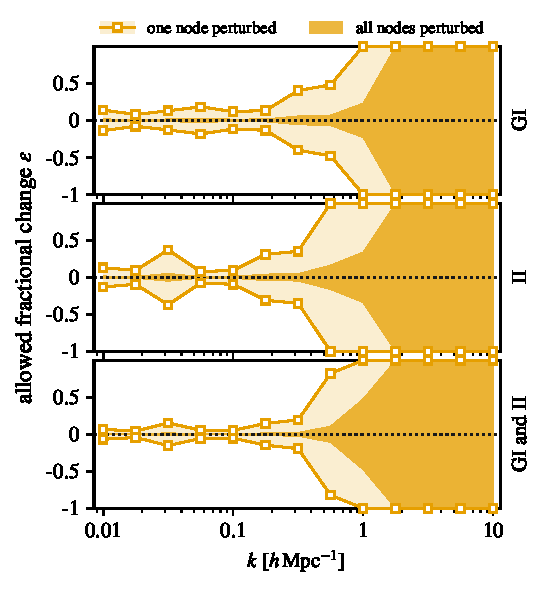
\includegraphics[width=3.5in]{plots/tolerance_bands_nla/tolerance_bands_nla.pdf}
  \caption{The fractional error $\varepsilon$ of the IA spectra that
    Roman tolerates at each scale, with NLA refitted. Light band with open
    markers: one node wrong, every other node exact; dark band: every node
    wrong at once, inside which every combination of signs and sizes keeps
    the figure of bias below 0.3. Panels: GI, II, and both changed by the
    same $\varepsilon$. The change is the same at every redshift. Mask
    $\kuv = 0.3/D(z)$, production covariance, $\Omega_m$ and $A_s$ free.}
  \label{fig:nla}
\end{figure}

\begin{figure}[tbp]
  \centering
  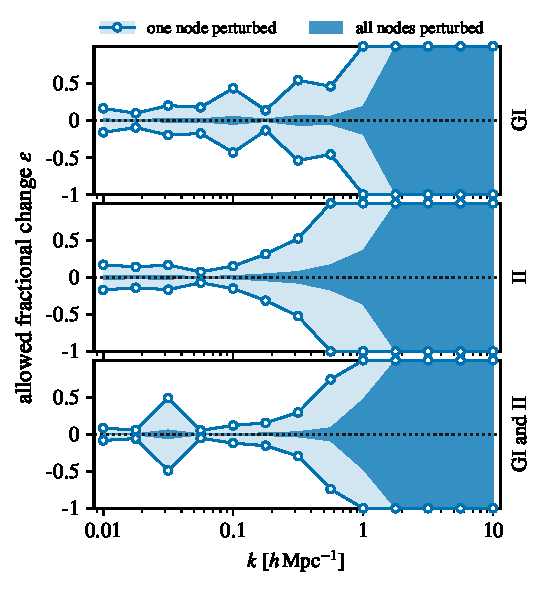
\includegraphics[width=3.5in]{plots/tolerance_bands_tatt/tolerance_bands_tatt.pdf}
  \caption{As Figure~\ref{fig:nla}, with TATT refitted.}
  \label{fig:tatt}
\end{figure}

\section{How the mask moves the bands}
\label{sec:masks}

Figure~\ref{fig:masks} repeats the guaranteed band for four production
masks, $K_0 = 0.2$ to 0.5, for GI and II wrong together, on a logarithmic
axis. A looser mask keeps more small-angle bins and so demands accuracy to
smaller scales: the edge where errors stop mattering moves from about $1
\hMpc$ ($K_0 = 0.2$) to about $3\hMpc$ ($K_0 = 0.5$), and the band at 0.1 to
$1\hMpc$ narrows by up to a factor of 15. On the largest scales, $k \lesssim
0.06\hMpc$, the band changes much less, by a factor of 1 to 4: those scales
feed the large-angle bins that every mask keeps.

\begin{figure}[tbp]
  \centering
  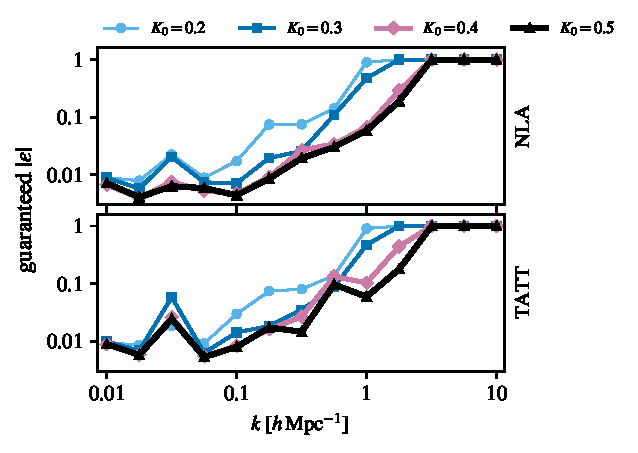
\includegraphics[width=3.5in]{plots/tolerance_masks/tolerance_masks.pdf}
  \caption{The guaranteed tolerance of GI and II changed together, for the
    production masks $\kuv = K_0/D(z)$, $K_0$ in $h\,{\rm Mpc}^{-1}$; the
    upper edge only, since the bands are symmetric. Color, line width and
    marker: the mask. Upper panel NLA, lower panel TATT; $\Omega_m$ and
    $A_s$ free.}
  \label{fig:masks}
\end{figure}

\section{Is linear response enough?}
\label{sec:verify}

Equation~\eqref{eq:response} predicts a figure of bias of exactly 0.3 at
every band edge. Figure~\ref{fig:verify} replaces it by full non-linear
refits at 16 edges per model on the $K_0 = 0.3$ mask: both signs at the
single-node edge of the three most sensitive nodes, and both worst-case
corners of the guaranteed box, for GI and for II. The shift is measured
from the refit of the unperturbed truth.

For NLA every refit lands between \VerNLAHi{} and \VerNLALo{}: the bands
are accurate to 8\%, slightly optimistic, and symmetric in sign within
3\%. For TATT the spread is wider, \VerTATTLo{} to \VerTATTHi, and one
corner gives \VerTATTCorner: TATT's parameters ($\eta_2$, $b_{\rm TA}$) sit
near their prior bounds and respond non-linearly, so with all nodes
perturbed the refit can reach a different part of its parameter space and
absorb more than the linear response predicts. Shrinking the bands by
10\% (NLA) or 20\% (TATT) makes them strictly safe.

Linear response fails without a scale cut. With all 1080 points, NLA
cannot describe the stitched truth ($\chi^2 = \AllChi$, figure of bias
\AllFoB{} before any perturbation), the neglected term $\sum_a (d -
m)_a\,\partial^2 m_a$ is large, and full refits at the predicted edges gave
figures of bias of 0.15 to 1.2. The bands are only meaningful on masks where
the model fits.

\begin{figure}[tbp]
  \centering
  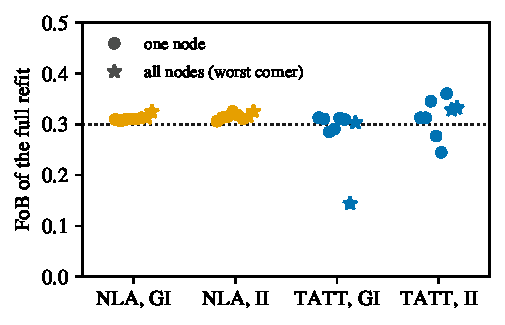
\includegraphics[width=3.5in]{plots/verification/verification.pdf}
  \caption{Full non-linear refits at the edges of the linear-response bands
    (mask $\kuv = 0.3/D(z)$, $\Omega_m$ and $A_s$ free), where linear
    response predicts 0.3 (dotted). Circles: one node at its edge, three
    nodes and both signs; stars: the two worst-case corners of the
    guaranteed box. NLA orange, TATT blue.}
  \label{fig:verify}
\end{figure}

\section{From tolerance to a scale cut}
\label{sec:cut}

The bands turn the choice of a scale cut into a comparison of two curves.
For a model with fractional error $\Delta_X(k) = P_X^{\rm model}/P_X^{\rm
true} - 1$, the mask is safe when $|\Delta_X(k)|$ stays inside the
guaranteed band of that mask at every node; the cut is the loosest mask for
which this holds. Two remarks for using it.
\begin{itemize}
  \item The bands bound the additional shift. The stitched truth already
    biases the refit by itself, with figures of bias of \BaseTwo,
    \BaseThree, \BaseFour{} and \BaseFive{} (NLA / TATT) at $K_0 = 0.2$,
    0.3, 0.4 and 0.5, because NLA and TATT do not describe the FLAMINGO
    side of the stitch. Shifts add as vectors, so a total budget of 0.3
    leaves $0.3 - \FoB_{\rm base}$ for further errors in the worst case,
    and the bands scale linearly with that remainder.
  \item The model error must be the error of the model as it is fitted,
    not at fixed amplitude: the response already lets $A_1$ and the other
    IA parameters move, so only the part of $\Delta_X$ that they cannot
    absorb matters.
\end{itemize}

\appendix

\section{Case B: more cosmological freedom}
\label{app:caseB}

With $n_s$, $H_0$ and $\Omega_b$ also free (Gaussian priors of the chain
width), $\sigma(S_8)$ grows by about 30\% and the same perturbation is a
smaller fraction of it. The guaranteed bands mostly widen, by up to a
factor of 5 at $k \le 0.1\hMpc$ (one node, $0.056\hMpc$, narrows), and are
similar above; the ratio of the guaranteed to
the single-node band stays at \RatioLo{} to \RatioHi. All case-B bands are in
the figures' \texttt{data.json} (key \texttt{case\_B}).

\section{Numerical checks}
\label{app:checks}

\begin{itemize}
  \item \textbf{Build.} cocoa-cosmolike-core and cocoa\_roman\_real (cocoa
    v5.x) with the two sim-IA patches of \texttt{cosmolike\_patches/},
    compiled with \texttt{-DSIM\_KMIN\_HMPC=1e-6 -DSIM\_KMAX\_HMPC=0}. The
    injected $\xi_{\rm IA}$ of the production and stitched truths agree with
    the earlier build to $\BuildCheck$ (largest difference over the largest
    value; median $2\times10^{-4}$), the difference of CAMB and cocoa
    versions.
  \item \textbf{Fitter.} The earlier stitched-truth test (Gaussian
    covariance, $K_0 = 0.3$, case A) is reproduced for NLA (0.279 against
    0.281). TATT lands in a different minimum (0.32 against 0.25, with
    $\eta_2$ and $b_{\rm TA}$ at their bounds): its likelihood has several.
  \item \textbf{Basis.} The node responses sum to $\bvec\xi_{\rm IA}$ to
    $\PartitionCheck$.
\end{itemize}

\section{Where the code and results are}
\label{app:code}

Paths relative to the repository root.

\begin{center}
  \small
  \begin{tabular}{ll}
    \toprule
    step & file \\
    \midrule
    responses, fits, bands, verification & \texttt{analysis/roman\_dchi2/v7/tolerance\_bands.py} \\
    results and log & \texttt{v7/tolerance\_bands.json}, \texttt{v7/tolerance\_bands\_log.txt} \\
    stitched truth & \texttt{analysis/roman\_dchi2/v3/stitched\_truths.npz} (variant S1) \\
    figure data & \texttt{notes/ia\_tolerance\_bands/plots/make\_figure\_data.py} \\
    \bottomrule
  \end{tabular}
\end{center}

\section{Open issues}
\label{app:open}

\begin{itemize}
  \item The perturbations are coherent in redshift. Errors that differ
    between redshifts form a larger space, which could give a stricter
    guaranteed band.
  \item The equal-share allocation of the guaranteed box is one choice
    among many; a band shaped like a model's expected error would be less
    conservative where that model is good.
  \item One truth (FLAMINGO, one galaxy selection, stitched to NLA); a
    different large-scale IA truth changes the arrows $\bvec L_j$ only
    through the best-fit point, but changes the baseline bias directly.
  \item The comparison of the bands with the actual NLA and TATT errors,
    which turns them into a cut (Section~\ref{sec:cut}), has not been made.
\end{itemize}

\end{document}
